\documentclass{standalone}
\usepackage{tikz}
\usetikzlibrary{patterns, positioning}

\begin{document}
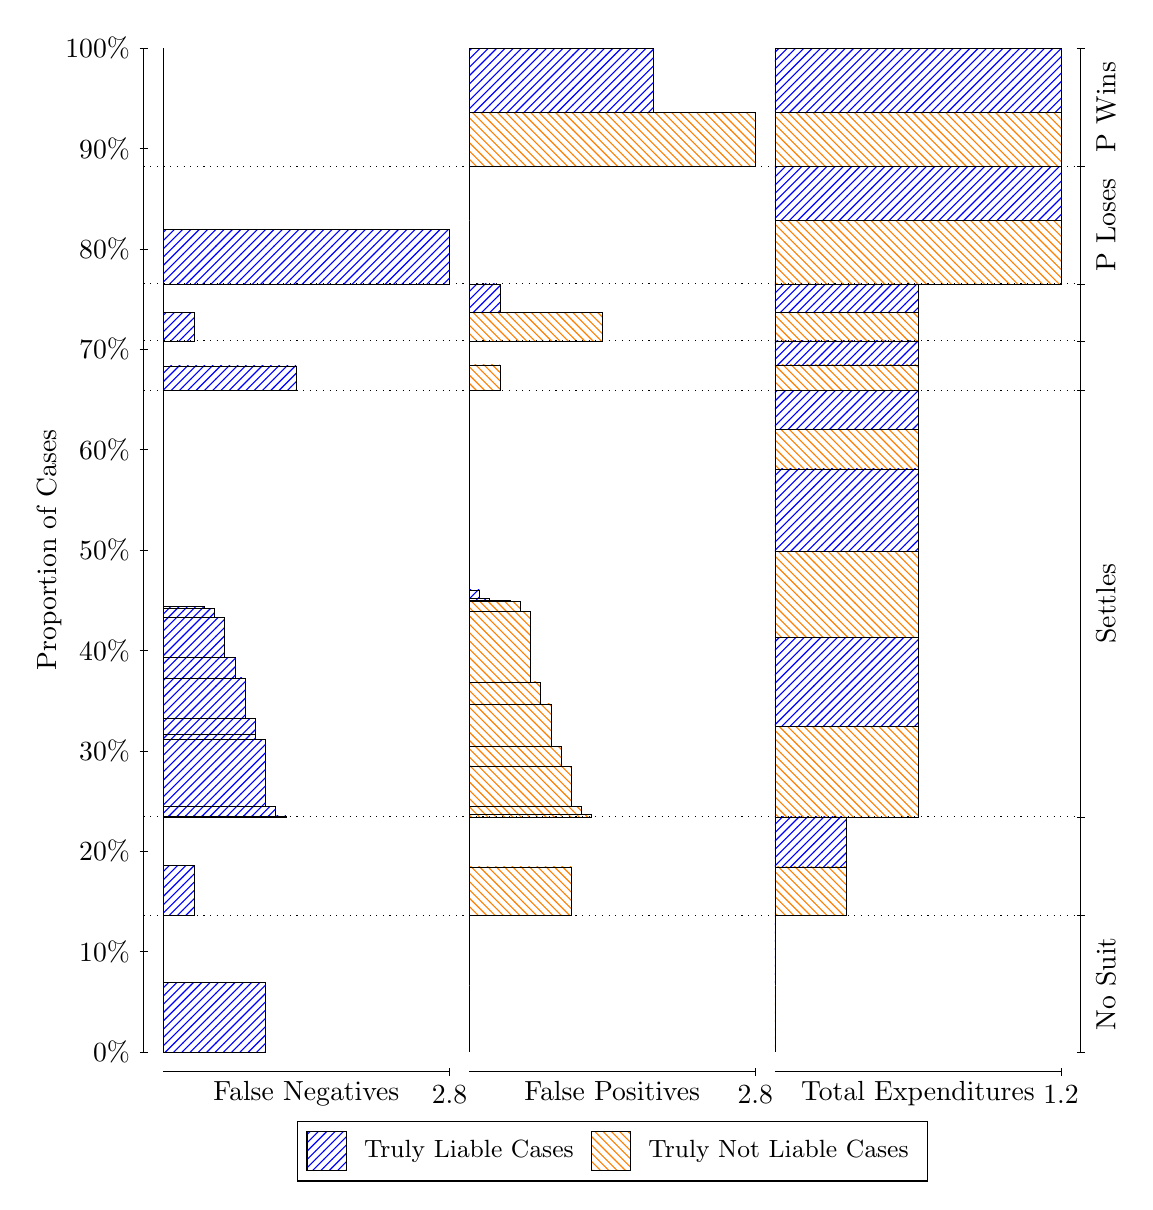
\begin{tikzpicture}
\draw[black, very thin] (1.5,1.75) -- (1.5,14.5);
\node[rotate=90, anchor=center] at (0.3, 8.125) {Proportion of Cases};
\draw[black, very thin] (1.45,1.75) -- (1.55,1.75);
\node[anchor=east] at (1.45, 1.75) {0\%};
\draw[black, very thin] (1.45,3.025) -- (1.55,3.025);
\node[anchor=east] at (1.45, 3.025) {10\%};
\draw[black, very thin] (1.45,4.3) -- (1.55,4.3);
\node[anchor=east] at (1.45, 4.3) {20\%};
\draw[black, very thin] (1.45,5.575) -- (1.55,5.575);
\node[anchor=east] at (1.45, 5.575) {30\%};
\draw[black, very thin] (1.45,6.85) -- (1.55,6.85);
\node[anchor=east] at (1.45, 6.85) {40\%};
\draw[black, very thin] (1.45,8.125) -- (1.55,8.125);
\node[anchor=east] at (1.45, 8.125) {50\%};
\draw[black, very thin] (1.45,9.4) -- (1.55,9.4);
\node[anchor=east] at (1.45, 9.4) {60\%};
\draw[black, very thin] (1.45,10.675) -- (1.55,10.675);
\node[anchor=east] at (1.45, 10.675) {70\%};
\draw[black, very thin] (1.45,11.95) -- (1.55,11.95);
\node[anchor=east] at (1.45, 11.95) {80\%};
\draw[black, very thin] (1.45,13.225) -- (1.55,13.225);
\node[anchor=east] at (1.45, 13.225) {90\%};
\draw[black, very thin] (1.45,14.5) -- (1.55,14.5);
\node[anchor=east] at (1.45, 14.5) {100\%};

\draw[black, very thin] (13.4,1.75) -- (13.4,14.5);
\draw[black, very thin] (13.35,1.75) -- (13.45,1.75);
\node[anchor=west] at (13.35, 1.75) {};
\draw[black, very thin] (13.35,3.4815) -- (13.45,3.4815);
\node[anchor=west] at (13.35, 3.4815) {};
\draw[black, very thin] (13.35,4.7352) -- (13.45,4.7352);
\node[anchor=west] at (13.35, 4.7352) {};
\draw[black, very thin] (13.35,10.156) -- (13.45,10.156);
\node[anchor=west] at (13.35, 10.156) {};
\draw[black, very thin] (13.35,10.781) -- (13.45,10.781);
\node[anchor=west] at (13.35, 10.781) {};
\draw[black, very thin] (13.35,11.506) -- (13.45,11.506);
\node[anchor=west] at (13.35, 11.506) {};
\draw[black, very thin] (13.35,13.001) -- (13.45,13.001);
\node[anchor=west] at (13.35, 13.001) {};
\draw[black, very thin] (13.35,14.5) -- (13.45,14.5);
\node[anchor=west] at (13.35, 14.5) {};

\draw[black, very thin, pattern color=blue, pattern=north east lines] (1.75,1.75) rectangle (3.0476,2.6363);
\draw[black, very thin, pattern color=orange, pattern=north west lines] (1.75,2.6363) rectangle (1.75,3.4815);
\draw[black, very thin, pattern color=blue, pattern=north east lines] (1.75,3.4815) rectangle (2.1393,4.1164);
\draw[black, very thin, pattern color=orange, pattern=north west lines] (1.75,4.1164) rectangle (1.75,4.7352);
\draw[black, very thin, pattern color=blue, pattern=north east lines] (1.75,4.7352) rectangle (3.3071,4.7491);
\draw[black, very thin, pattern color=blue, pattern=north east lines] (1.75,4.7491) rectangle (3.1774,4.8656);
\draw[black, very thin, pattern color=blue, pattern=north east lines] (1.75,4.8656) rectangle (3.0476,5.7204);
\draw[black, very thin, pattern color=blue, pattern=north east lines] (1.75,5.7204) rectangle (2.9179,5.7798);
\draw[black, very thin, pattern color=blue, pattern=north east lines] (1.75,5.7798) rectangle (2.9179,5.9863);
\draw[black, very thin, pattern color=blue, pattern=north east lines] (1.75,5.9863) rectangle (2.7881,6.5017);
\draw[black, very thin, pattern color=blue, pattern=north east lines] (1.75,6.5017) rectangle (2.6583,6.7634);
\draw[black, very thin, pattern color=blue, pattern=north east lines] (1.75,6.7634) rectangle (2.5286,7.2721);
\draw[black, very thin, pattern color=blue, pattern=north east lines] (1.75,7.2721) rectangle (2.3988,7.3808);
\draw[black, very thin, pattern color=blue, pattern=north east lines] (1.75,7.3808) rectangle (2.269,7.4093);
\draw[black, very thin, pattern color=orange, pattern=north west lines] (1.75,7.4093) rectangle (1.75,10.156);
\draw[black, very thin, pattern color=blue, pattern=north east lines] (1.75,10.156) rectangle (3.4369,10.462);
\draw[black, very thin, pattern color=orange, pattern=north west lines] (1.75,10.462) rectangle (1.75,10.781);
\draw[black, very thin, pattern color=blue, pattern=north east lines] (1.75,10.781) rectangle (2.1393,11.147);
\draw[black, very thin, pattern color=orange, pattern=north west lines] (1.75,11.147) rectangle (1.75,11.506);
\draw[black, very thin, pattern color=blue, pattern=north east lines] (1.75,11.506) rectangle (5.3833,12.198);
\draw[black, very thin, pattern color=orange, pattern=north west lines] (1.75,12.198) rectangle (1.75,13.001);
\draw[black, very thin, pattern color=orange, pattern=north west lines] (1.75,13.001) rectangle (1.75,13.685);
\draw[black, very thin, pattern color=blue, pattern=north east lines] (1.75,13.685) rectangle (1.75,14.5);
\draw[black, very thin, pattern color=orange, pattern=north west lines] (5.6333,1.75) rectangle (5.6333,2.5953);
\draw[black, very thin, pattern color=blue, pattern=north east lines] (5.6333,2.5953) rectangle (5.6333,3.4815);
\draw[black, very thin, pattern color=orange, pattern=north west lines] (5.6333,3.4815) rectangle (6.931,4.1003);
\draw[black, very thin, pattern color=blue, pattern=north east lines] (5.6333,4.1003) rectangle (5.6333,4.7352);
\draw[black, very thin, pattern color=orange, pattern=north west lines] (5.6333,4.7352) rectangle (7.1905,4.7628);
\draw[black, very thin, pattern color=orange, pattern=north west lines] (5.6333,4.7628) rectangle (7.0607,4.8673);
\draw[black, very thin, pattern color=orange, pattern=north west lines] (5.6333,4.8673) rectangle (6.931,5.3731);
\draw[black, very thin, pattern color=orange, pattern=north west lines] (5.6333,5.3731) rectangle (6.8012,5.6355);
\draw[black, very thin, pattern color=orange, pattern=north west lines] (5.6333,5.6355) rectangle (6.6714,6.171);
\draw[black, very thin, pattern color=orange, pattern=north west lines] (5.6333,6.171) rectangle (6.5417,6.4497);
\draw[black, very thin, pattern color=orange, pattern=north west lines] (5.6333,6.4497) rectangle (6.4119,7.3435);
\draw[black, very thin, pattern color=orange, pattern=north west lines] (5.6333,7.3435) rectangle (6.2821,7.4676);
\draw[black, very thin, pattern color=orange, pattern=north west lines] (5.6333,7.4676) rectangle (6.1524,7.482);
\draw[black, very thin, pattern color=blue, pattern=north east lines] (5.6333,7.482) rectangle (5.8929,7.5105);
\draw[black, very thin, pattern color=blue, pattern=north east lines] (5.6333,7.5105) rectangle (5.7631,7.6192);
\draw[black, very thin, pattern color=blue, pattern=north east lines] (5.6333,7.6192) rectangle (5.6333,10.156);
\draw[black, very thin, pattern color=orange, pattern=north west lines] (5.6333,10.156) rectangle (6.0226,10.475);
\draw[black, very thin, pattern color=blue, pattern=north east lines] (5.6333,10.475) rectangle (5.6333,10.781);
\draw[black, very thin, pattern color=orange, pattern=north west lines] (5.6333,10.781) rectangle (7.3202,11.14);
\draw[black, very thin, pattern color=blue, pattern=north east lines] (5.6333,11.14) rectangle (6.0226,11.506);
\draw[black, very thin, pattern color=orange, pattern=north west lines] (5.6333,11.506) rectangle (5.6333,12.309);
\draw[black, very thin, pattern color=blue, pattern=north east lines] (5.6333,12.309) rectangle (5.6333,13.001);
\draw[black, very thin, pattern color=orange, pattern=north west lines] (5.6333,13.001) rectangle (9.2667,13.685);
\draw[black, very thin, pattern color=blue, pattern=north east lines] (5.6333,13.685) rectangle (7.969,14.5);
\draw[black, very thin, pattern color=orange, pattern=north west lines] (9.5167,1.75) rectangle (9.5167,2.5953);
\draw[black, very thin, pattern color=blue, pattern=north east lines] (9.5167,2.5953) rectangle (9.5167,3.4815);
\draw[black, very thin, pattern color=orange, pattern=north west lines] (9.5167,3.4815) rectangle (10.425,4.1003);
\draw[black, very thin, pattern color=blue, pattern=north east lines] (9.5167,4.1003) rectangle (10.425,4.7352);
\draw[black, very thin, pattern color=orange, pattern=north west lines] (9.5167,4.7352) rectangle (11.333,5.881);
\draw[black, very thin, pattern color=blue, pattern=north east lines] (9.5167,5.881) rectangle (11.333,7.0139);
\draw[black, very thin, pattern color=orange, pattern=north west lines] (9.5167,7.0139) rectangle (11.333,8.1096);
\draw[black, very thin, pattern color=blue, pattern=north east lines] (9.5167,8.1096) rectangle (11.333,9.1542);
\draw[black, very thin, pattern color=orange, pattern=north west lines] (9.5167,9.1542) rectangle (11.333,9.6594);
\draw[black, very thin, pattern color=blue, pattern=north east lines] (9.5167,9.6594) rectangle (11.333,10.156);
\draw[black, very thin, pattern color=orange, pattern=north west lines] (9.5167,10.156) rectangle (11.333,10.475);
\draw[black, very thin, pattern color=blue, pattern=north east lines] (9.5167,10.475) rectangle (11.333,10.781);
\draw[black, very thin, pattern color=orange, pattern=north west lines] (9.5167,10.781) rectangle (11.333,11.14);
\draw[black, very thin, pattern color=blue, pattern=north east lines] (9.5167,11.14) rectangle (11.333,11.506);
\draw[black, very thin, pattern color=orange, pattern=north west lines] (9.5167,11.506) rectangle (13.15,12.309);
\draw[black, very thin, pattern color=blue, pattern=north east lines] (9.5167,12.309) rectangle (13.15,13.001);
\draw[black, very thin, pattern color=orange, pattern=north west lines] (9.5167,13.001) rectangle (13.15,13.685);
\draw[black, very thin, pattern color=blue, pattern=north east lines] (9.5167,13.685) rectangle (13.15,14.5);
\draw[black, dotted] (1.5,3.4815) -- (13.4,3.4815);
\draw[black, dotted] (1.5,4.7352) -- (13.4,4.7352);
\draw[black, dotted] (1.5,10.156) -- (13.4,10.156);
\draw[black, dotted] (1.5,10.781) -- (13.4,10.781);
\draw[black, dotted] (1.5,11.506) -- (13.4,11.506);
\draw[black, dotted] (1.5,13.001) -- (13.4,13.001);
\draw[black, very thin] (1.75,1.5) -- (5.3833,1.5);
\node[anchor=north] at (3.5667, 1.5) {False Negatives};
\draw[black, very thin] (5.3833,1.45) -- (5.3833,1.55);
\node[anchor=north] at (5.3833, 1.45) {2.8};

\draw[black, very thin] (5.6333,1.5) -- (9.2667,1.5);
\node[anchor=north] at (7.45, 1.5) {False Positives};
\draw[black, very thin] (9.2667,1.45) -- (9.2667,1.55);
\node[anchor=north] at (9.2667, 1.45) {2.8};

\draw[black, very thin] (9.5167,1.5) -- (13.15,1.5);
\node[anchor=north] at (11.333, 1.5) {Total Expenditures};
\draw[black, very thin] (13.15,1.45) -- (13.15,1.55);
\node[anchor=north] at (13.15, 1.45) {1.2};

\node[black, centered, rotate=90] at (13.72, 2.6158) {No Suit};

\node[black, centered, rotate=90] at (13.72, 7.4456) {Settles};


\node[black, centered, rotate=90] at (13.72, 12.253) {P Loses};
\node[black, centered, rotate=90] at (13.72, 13.751) {P Wins};

\draw (7.449999999999999,1.5) node[draw=none] (baseCoordinate) {};
\begin{scope}[align=center]
        \matrix[scale=0.5, draw=black, below=0.5cm of baseCoordinate, nodes={draw}, column sep=0.1cm]{
            \node[rectangle, draw, minimum width=0.5cm, minimum height=0.5cm, pattern=north east lines, pattern color=blue] {}; &
            \node[draw=none, font=\small] (B) {Truly Liable Cases}; &
            \node[rectangle, draw, minimum width=0.5cm, minimum height=0.5cm, pattern=north west lines, pattern color=orange] {}; &
            \node[draw=none, font=\small] (B) {Truly Not Liable Cases}; \\
            };
\end{scope}

\end{tikzpicture}
\end{document}